\section{Circuits} 
\begin{figure} 
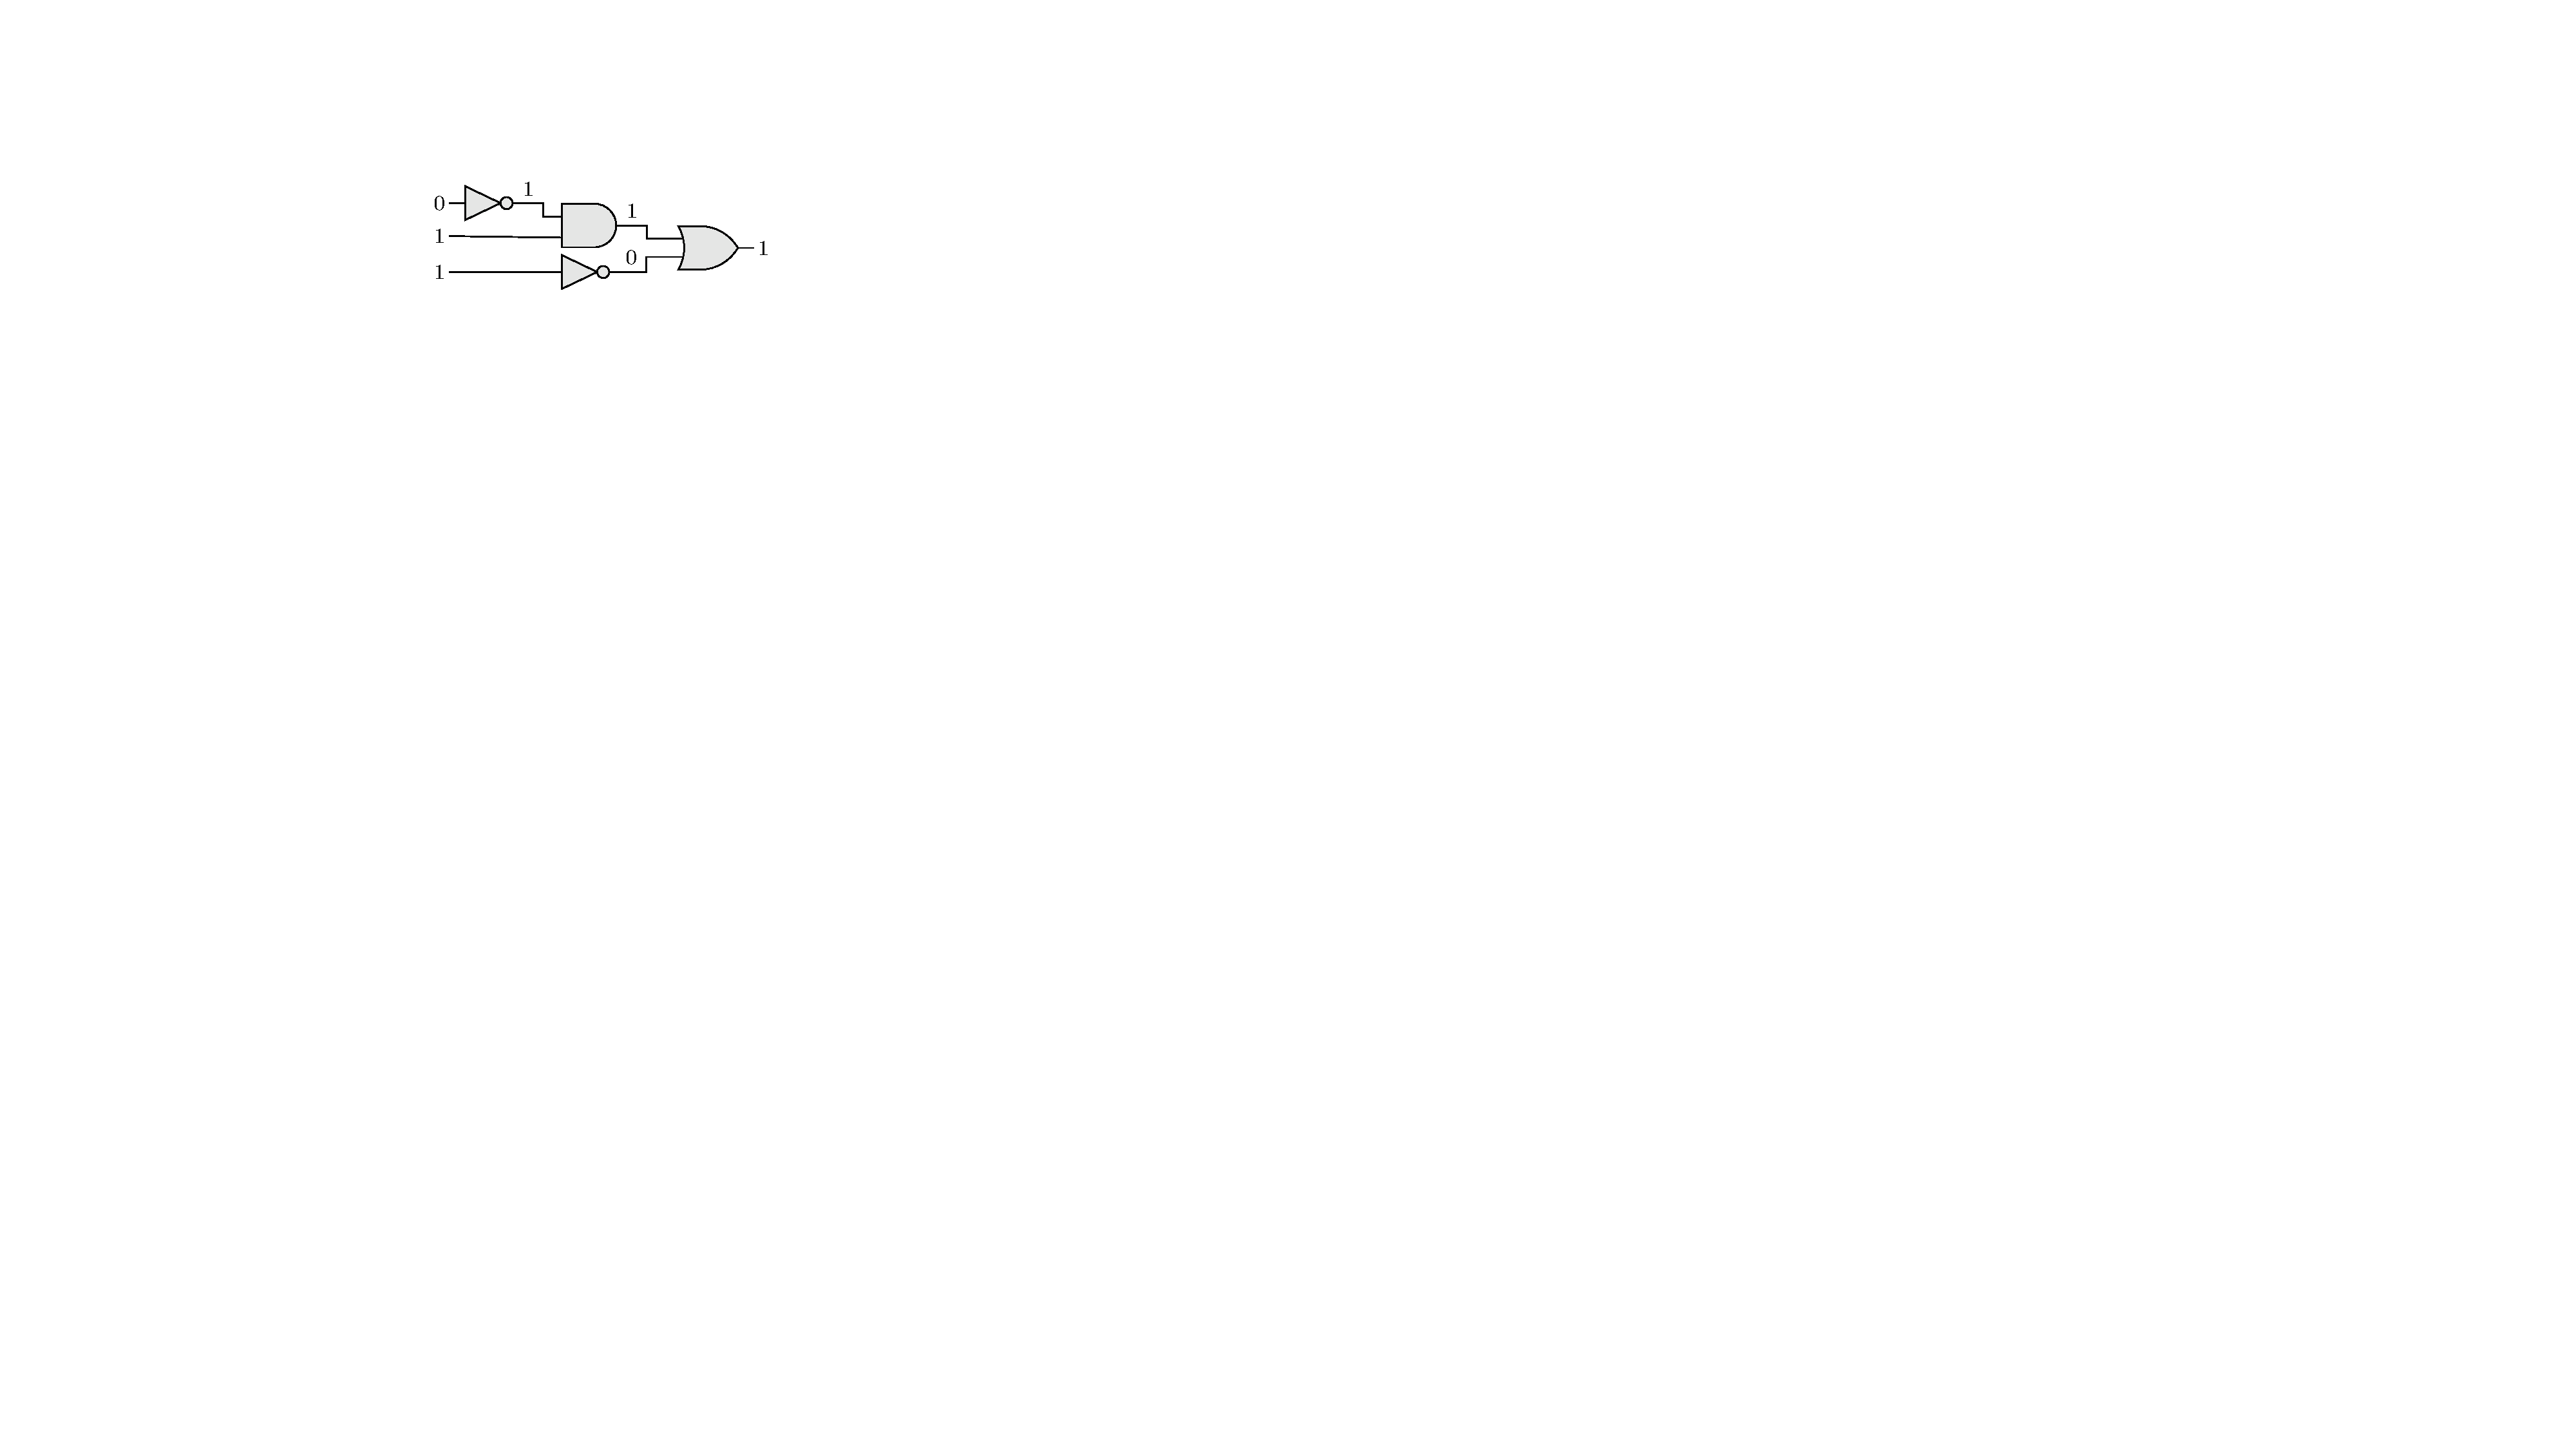
\includegraphics[]{Figures/HWCircuits/DigitalCircuit} 
\end{figure}

\newcommand\bstate{b}
\newcommand\qustate{q}

\paragraph{Bits and Qubits}
In classical computing, bits are the fundamental units of information. 
%
They can exist in only one of two possible states: 0 or 1. 
%
They may be conceptualized as switches that are either turned on or off. 
%
In contrast, quantum computing employs quantum bits, known as {\it qubits}, to represent and process information. 
%
Qubits can exist in a {\it superposition}, meaning they can be in state 0, state 1, or a combination of both simultaneously. 
%
Furthermore, a qubit can undergo a {\it measurement} process. 
%
A qubit’s state can be described by two complex numbers, called {\it amplitudes}, $c_0$ and $c_1$, where $|c_0|^2$ represents the probability of measuring the state as $0$, and $|c_1|^2$ the probability of measuring it as $1$. 
%
We require that $|c_0|^2 + |c_1|^2 = 1$.

There are two common representations used to describe a qubit state.
%
One is the vector notation, where the state is written as a column vector of length 2 (see \cref{qbit:column:fig}) with complex entries corresponding to the amplitudes of the respective basis states.
%
To simplify notation, we often use the transpose of the column vector.
%
This results in a row vector, which is more compact and easier to write.
%
As a special case, we may refer directly to standard basis column vectors.
%
The second representation is the Dirac notation, where the state is expressed as $c_0|0\rangle + c_1|1\rangle$.
%
The classical states are special cases where either $c_0=1$ and $c_1=0$ or
$c_0=0$ and $c_1=1$.
%
In the contrext of quantum systems, we refer to theses states as the basis states $|0\rangle$ and $|1\rangle$.

We genberalize the above concepts to the case where we have multiple qubits.
%
For $n$ bits we have $2^n$ states.
%
For instance, when $n=2$, we have four basis states $00,01,10,11$, and a quantum state is of the form $c_{00}|00\rangle+c_{01}|01\rangle+c_{10}|0\rangle+c_{11}|11\rangle$

The concepts
Superposition allows quantum circuits to encode information more efficiently than classical circuits. 
%
Furthermore, qubits can be {\it entangled}: the state of one qubit is connected to another. 
%
Entaglement means the state of one qubit can't be described independently of the others.
%
The state of one qbit may be possible to derive from the state of another qubit, even if when physicallyu far away.

We will represent qu(bits) by  (column) matrices
\[
\left[
\begin{array}{c}
0\\1
\end{array}
\right]
\;\;\;
\left[
\begin{array}{c}
1\\0
\end{array}
\right]
\;\;\;
\left[
\begin{array}{c}
\sqrt{\frac1 2}\\\\\sqrt{\frac1 2}
\end{array}
\right]
\;\;\;
\left[
\begin{array}{c}
\frac1 3\\\\\frac{\sqrt8}3
\end{array}
\right]
\;\;\;
\left[
\begin{array}{c}
c_0\\\\c_1
\end{array}
\right]
\left[
c_0\;\;\;c_1
\right]^{\mathtt T}
\]

More egenrally, we will work with multiple (qu)bits.
%
In the case where we have two qubits the systems wiill have four states.
%
The basis states are given by 
\[
\left[
1\;0\;0\;0
\right]^{\mathtt T}
\;\;\;
\left[
0\;\;1\;0\;0
\right]^{\mathtt T}
\;\;\;
\left[
0\;0\;1\;0
\right]^{\mathtt T}
\;\;\;
\left[
0\;0\;0\;1
\right]^{\mathtt T}
\]
A quantum state will have the form
\[
\left[
c_0\;\;c_1\;\;c_2\;\;c_3
\right]^{\mathtt T}
\;\;\;
\left[
\frac1 4\;\;\frac 3 4\;\;\frac 1 {\sqrt8}\;\;\frac 1 2
\right]^{\mathtt T}
\]


\paragraph{Gates}
Logical gates, such as AND, OR, and NOT, are the fundamental components of digital circuits. 
%
They take binary inputs (0s and 1s) and produce a single binary output.
%
Each type of gate implements a specific binary function, e.g., the output of an AND gate is the conjunction of its inputs.
%
Quantum gates like the Hadamard and CNOT are the building blocks of quantum circuits, similar to classical logic gates. They manipulate qubits through unitary operations, allowing for quantum algorithms. Each gate performs a specific transformation, enabling superposition, entanglement, and measurement, thus enabling more complex computations compared to classical gates.

\paragraph{States}
The state of a sequence of bits is often represented by listing their values. For example, the input state in the figure is 011, indicating the values of the three input bits. Generally, $n$ bits can have $2^n$ possible states. 
%

In quantum computing, bits and states have a richer structure.
%
A {\it basis state} for a quantum bit is one of the classical states $0$ or $1$.
%
A qubit can be in a basis state or, more generally, in a {\it superposition} of the basis states, represented mathematically as: $[|\psi⟩ = \alpha |0⟩ + \beta |1⟩ ]$.
Here, $\alpha$ and $\beta$ are complex coefficients that determine the probability of measuring the qubit in either state.
The probabilities are given by:
Probability of measuring $|0⟩$: $( |\alpha|^2 )$
Probability of measuring $|1⟩$: $( |\beta|^2 )$
The condition $( |\alpha|^2 + |\beta|^2 = 1 )$ must hold to ensure valid probabilities.
%
In a system with $\nn$ qubits, there are $2^\nn$ possible basis states.
%
In general, a quantum state is a superposition of a set of basis state, representing a probability distribution over the possible $2^n$ bit-assignments.
%
A quantum state $\qustate$ assignes to each basis state $\bstate$ a complex number $\alpha_\bstate$ called the {\it amplitude} of $\bstate$ in $\qustate$.
%
Intuitively, if we \patodo{measure} $\qustate$ then the probability that we observe $\bstate$ is given by the square $\alpha_\bstate^2$ iof thbe amplitude.
%
The a
The left side of \cref{qustate:tree:fig} shows a quantum state with three qubits.
%
Each row of the table gives the amplitude of one basis state.
%


\paragraph{Circuits}
A combinatorial circuit consists of a set of gates and acts as a Boolean function. It takes a sequence of bits as input and produces a sequence of bits as output. There are also internal bits that represent the connections between gates. In the figure, the circuit has three input bits, one output bit, and three internal bits.
\patodo{Describe quantum states}


The basis states represent the simplest forms of qubit states:
|0⟩: Represents the state where the qubit is definitively in the "0" position.
|1⟩: Represents the state where the qubit is definitively in the "1" position.
These states are often referred to as computational basis states.
3. Superposition

